\documentclass{article}
\usepackage{tikz, comment}
\usepackage{pifont}
\usepackage{fontspec, pgfplots}
\usetikzlibrary{arrows, decorations.markings, decorations.pathreplacing}
\begin{comment}
:Title: Not defined yet
:Tags: tangent line;directrix of a parabola;moment;focus of a parabola;parabola
:Prob: 0.5782;0.5271;0.523;0.5201;0.5106
:Author: Prof.Hu Ji-shan, HKUST
:Slug: No name yet

Description Here.........
\end{comment}
\begin{document}\centering 

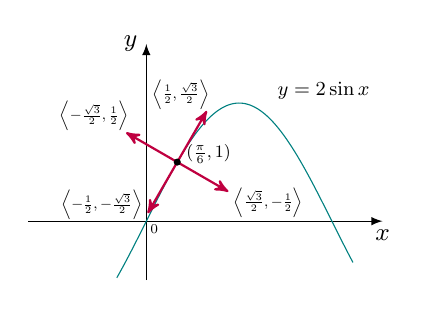
\begin{tikzpicture}[>=latex,xscale=.5*1.5, yscale=.5*1.5][font=\sf\small] 

\draw[->] (-2, 0) -- (4, 0)node[below] {$x$} ;
\draw[->] (0, -1) -- (0, 3)node[left] {$y$} ;

\clip[] (-2, -1) rectangle (4, 3);
\draw[teal, samples=100, smooth, domain=-0.5:3.5, variable=\x] 
		plot ({\x}, {2*sin(\x r)}); 

\draw [purple, thick, <->, >=stealth'] ({-1/2+pi/6}, {-sqrt(3)/2+1}) -- ({1/2+pi/6}, {sqrt(3)/2+1});

\draw [purple, thick, <->, >=stealth'] ({-sqrt(3)/2+pi/6}, {1/2+1}) -- ({sqrt(3)/2+pi/6}, {-1/2+1});

\node[left, xshift=0, yshift=3, scale=0.6] at ({-1/2+pi/6}, {-sqrt(3)/2+1}) {$\left\langle -\frac{1}{2}, - \frac{\sqrt 3}{2} \right\rangle$};

\node[left, xshift=3, yshift=6, scale=0.6] at ({1/2+pi/6}, {sqrt(3)/2+1}) {$\left\langle \frac{1}{2},  \frac{\sqrt 3}{2} \right\rangle$};

\node[left, xshift=3, yshift=6, scale=0.6] at ({-sqrt(3)/2+pi/6}, {1/2+1}) {$\left\langle -\frac{\sqrt 3}{2},  \frac{1}{2} \right\rangle$};

\node[right, xshift=0, yshift=-4, scale=0.6] at ({sqrt(3)/2+pi/6}, {-1/2+1}) {$\left\langle \frac{\sqrt 3}{2},  -\frac{1}{2} \right\rangle$};

\node[scale=0.8]  at (3, 2.2) {$y=2\sin x$};

\draw[fill] ({pi/6},1) circle(0.05)node[right, xshift=1, yshift=3, scale=0.7] {$(\frac{\pi}{6}, 1)$};

\node[scale=0.7] at (0.2/1.5, -0.2/1.5) {\scriptsize$0$};

\end{tikzpicture}
\end{document}